\section{Introduction}
Machine-learned interatomic potentials approximate a reference potential-energy
surface at a cost that permits molecular-dynamics (MD) sampling beyond typical
first-principles trajectories. Their usefulness depends on the environments
represented by the training data. A model can perform adequately on familiar
structures yet make consequential force errors when a trajectory reaches
an unfamiliar local arrangement. Active learning addresses this problem
by deciding where reference calculations should be added and incorporating
the resulting data into subsequent models. D-optimality-based selection
for moment tensor potentials and Bayesian on-the-fly force fields provide
established examples of this strategy
\citep{podryabinkin2017active,vandermause2020flare}.

An operational active-learning system also has to connect exploration,
reference labeling, and training. DP-GEN implements this cycle through
modular simulation and labeling backends \citep{zhang2020dpgen}.
For a large parent structure, however, even a single whole-system reference
calculation may be expensive. Local selection offers an additional way to
control this cost. Hodapp and Shapeev identify extrapolative subregions and
construct small periodic reference systems \citep{hodapp2020inoperando};
MLIP-3 supports active learning on atomic neighborhoods
\citep{podryabinkin2023mlip3}. Thus neither the closed loop nor the principle
of local active learning is introduced here.

Covalently connected molecules make the validity of local labels particularly
important. Cutting out a neighborhood changes its electronic environment and
can create unsaturated bonds. Hydrogen termination restores a closed-shell
fragment for the alkane systems considered here, but it does not guarantee
that all fragment forces equal their parent counterparts. Boundary atoms and
artificial caps can therefore require different treatment from the region
whose force is intended to be learned. A second, distinct issue is that the
learned model itself may depend on an environment larger than the retained
fragment. Reliable use of local supervision requires these two questions to
be kept separate.

This work presents the Physics-aware Hotspot Active Learning Platform
(PHAL) as implemented in GMD\_active. PHAL connects the GMD MD engine,
CP2K density-functional theory (DFT) calculations, and the GMD\_SGT
potential-training backend. The central implementation choices are staged
heuristic monitoring, event-based localization, explicit fragment-fidelity
checks, role-dependent force weights, and persistent workflow state.
GMD and GMD\_SGT denote the dynamics and training components of the
ecosystem; GMD\_active owns the active-learning logic.

We evaluate three questions using completed alkane pilot experiments:
whether capped fragments reproduce parent core forces within stated
tolerances; whether the software executes acquisition, labeling, and training
with traceable costs; and whether a real closed loop changes model error
and short-trajectory behavior. We retain unsuccessful configurations and
unexercised acquisition cases. The results support the feasibility of local
supervision and the operation of the implementation. They do not establish
that PHAL is a generally better acquisition policy or that its physical
features provide calibrated uncertainty.

\begin{figure}[tb]
  \centering
  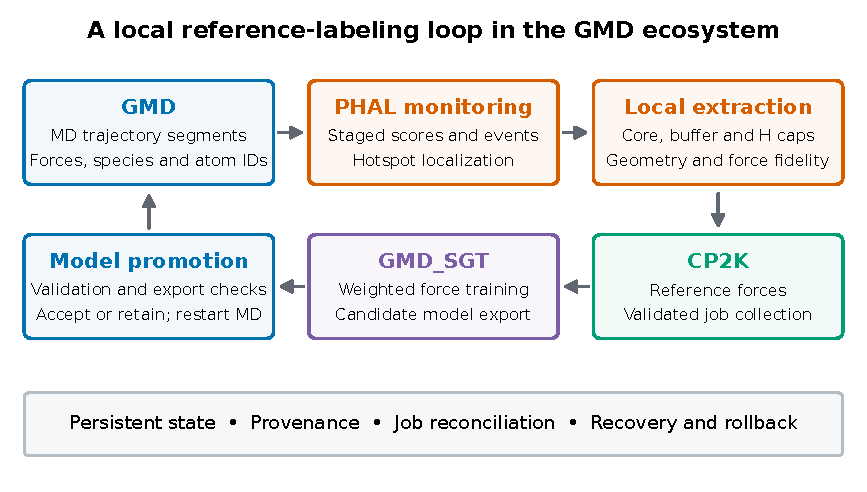
\includegraphics[width=\linewidth]{figures/fig01_workflow.pdf}
  \caption{PHAL within the GMD ecosystem. GMD produces trajectory segments;
  GMD\_active performs monitoring, extraction, job orchestration, and model
  promotion; CP2K provides reference labels; and GMD\_SGT trains and exports
  candidate models. Persistent records connect events, labels, datasets, and
  model versions. The diagram describes software responsibilities, not a
  guarantee that every candidate will be labeled or every trained model
  promoted.}
  \label{fig:workflow}
\end{figure}
